\documentclass[a4paper, 10pt]{article}
    \usepackage[subpreambles=true]{standalone}
    \usepackage[english, american, british]{babel}
    \usepackage[utf8]{inputenc}
    \usepackage[T1]{fontenc}
    \usepackage{hyphenat}
    \hyphenation{Mathe-matik wieder-gewinnen}
    \usepackage{amsmath}
    \usepackage{import}
    \usepackage{tabularx}
    \usepackage{graphicx}
    \usepackage{makecell}
    \usepackage{verbatim}
    \usepackage[margin=1cm ]{geometry}

    \title{Einführung in die Softwaretechnik 2018 \\ Sheet 07}
    \author{Maximilian Frühauf}

\begin{document}
\maketitle
\begin{enumerate}
    \setcounter{enumi}{3}
    \item
    Have a look at the example of Lecture 07 on slides 56 - 60. We already covered task 1 and task 2 , slide 59. In this exercise, you should solve:
    \begin{itemize}
        \item Task 3: Reverse engineer an analysis object model (UML class diagram) from the
    table where you group related attributes to the appropriate classes (e.g. car,
    location, temperature, battery, etc.)
        \item Task 4 (optional challenge): Create a small application to visualize the route with
    its source and destination (e.g. using a charts framework and Google Maps). Upload your solution as zip file to Moodle.
    \end{itemize}
    \vspace{0.5cm} 

    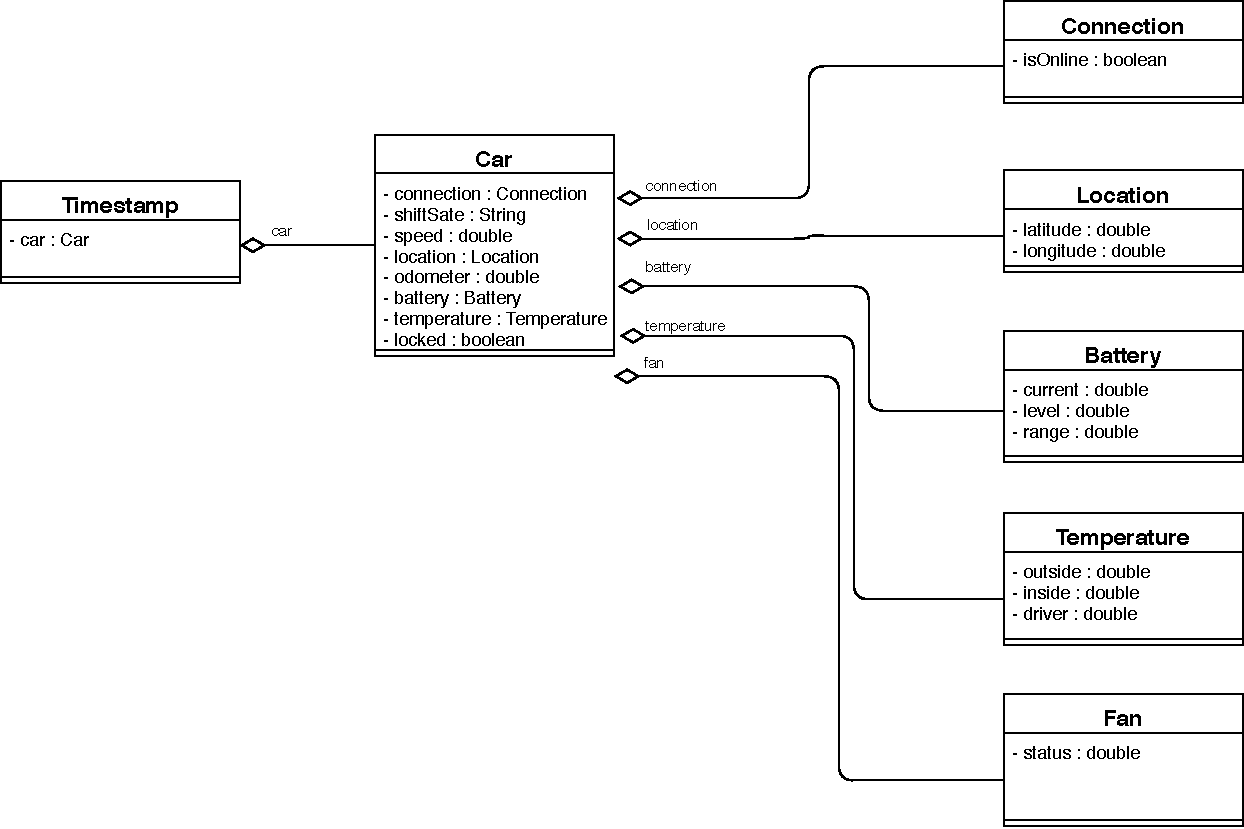
\includegraphics[width=\linewidth]{Task03.pdf}

    Bonus Task:

    To run the compiled \verb+.jar+ file, type into your console:
    \begin{verbatim}
        $ java -jar out/artifacts/mapViewer_jar/mapViewer.jar
    \end{verbatim}

    Or just execute the \verb+run.sh+ script:
    \begin{verbatim}
        $ chmod +x run.sh
        $ ./run.sh
    \end{verbatim}
\end{enumerate}
\end{document}